%%%%%%%%%%%%%%%%%%%%%%%%%%%%%%%%%%%%%%%%%%%%%%
% An example of a lab report write-up.
%%%%%%%%%%%%%%%%%%%%%%%%%%%%%%%%%%%%%%%%%%%%%%
% This is a combination of several labs that I have done in the past for
% Computer Engineering, so it is not to be taken literally, but instead used as
% a great starting template for your own lab write up.  When creating this
% template, I tried to keep in mind all of the functions and functionality of
% LaTeX that I spent a lot of time researching and using in my lab reports and
% include them here so that it is fairly easy for students first learning LaTeX
% to jump on in and get immediate results.  However, I do assume that the
% person using this guide has already created at least a "Hello World" PDF
% document using LaTeX (which means it's installed and ready to go).
%
% My preference for developing in LaTeX is to use the LaTeX Plugin for gedit in
% Linux.  There are others for Mac and Windows as well (particularly MikTeX).
% Another excellent plugin is the Calc2LaTeX plugin for the OpenOffice suite.
% It makes it very easy to create a large table very quickly.
%
% Professors have different tastes for how they want the lab write-ups done, so
% check with the section layout for your class and create a template file for
% each class (my recommendation).
%
% Also, there is a list of common commands at the bottom of this document.  Use
% these as a quick reference.  If you'd like more, you can view the "LaTeX Cheat
% Sheet.pdf" included with this template material.
%
% (c) 2009 Derek R. Hildreth <derek@derekhildreth.com> http://www.derekhildreth.com
% This work is licensed under the Creative Commons Attribution-NonCommercial-ShareAlike License. To view a copy of this license, visit http://creativecommons.org/licenses/by-nc-sa/1.0/ or send a letter to Creative Commons, 559 Nathan Abbott Way, Stanford, California 94305, USA.
%%%%%%%%%%%%%%%%%%%%%%%%%%%%%%%%%%%%%%%%%%%%%%
\documentclass[aps,letterpaper,10pt]{revtex4}
\input kvmacros % For Karnaugh Maps (K-Maps)

\usepackage{graphicx} % For images
\usepackage{float}    % For tables and other floats
\usepackage{verbatim} % For comments and other
\usepackage{amsmath}  % For math
\usepackage{amssymb}  % For more math
\usepackage{fullpage} % Set margins and place page numbers at bottom center
\usepackage{listings} % For source code
\usepackage{subfig}   % For subfigures
\usepackage[usenames,dvipsnames]{color} % For colors and names
\usepackage{hyperref}           % For hyperlinks and indexing the PDF
\usepackage{listings}
\usepackage{color}

\definecolor{dkgreen}{rgb}{0,0.6,0}
\definecolor{gray}{rgb}{0.5,0.5,0.5}
\definecolor{mauve}{rgb}{0.58,0,0.82}

\newcommand{\RNum}[1]{\uppercase\expandafter{\romannumeral #1\relax}}

\lstset{frame=tb,
  language=Python,
  aboveskip=3mm,
  belowskip=3mm,
  showstringspaces=false,
  columns=flexible,
  basicstyle={\small\ttfamily},
  numbers=none,
  numberstyle=\tiny\color{gray},
  keywordstyle=\color{blue},
  commentstyle=\color{dkgreen},
  stringstyle=\color{mauve},
  breaklines=true,
  breakatwhitespace=true,
  tabsize=3
}
%==========================================================================
\hypersetup{ % play with the different link colors here
    colorlinks,
    citecolor=blue,
    filecolor=blue,
    linkcolor=blue,
    urlcolor=blue % set to black to prevent printing blue links
}

\definecolor{mygrey}{gray}{.96} % Light Grey
\lstset{
	language=[ISO]C++,              % choose the language of the code ("language=Verilog" is popular as well)
   tabsize=3,							  % sets the size of the tabs in spaces (1 Tab is replaced with 3 spaces)
	basicstyle=\tiny,               % the size of the fonts that are used for the code
	numbers=left,                   % where to put the line-numbers
	numberstyle=\tiny,              % the size of the fonts that are used for the line-numbers
	stepnumber=2,                   % the step between two line-numbers. If it's 1 each line will be numbered
	numbersep=5pt,                  % how far the line-numbers are from the code
	backgroundcolor=\color{mygrey}, % choose the background color. You must add \usepackage{color}
	%showspaces=false,              % show spaces adding particular underscores
	%showstringspaces=false,        % underline spaces within strings
	%showtabs=false,                % show tabs within strings adding particular underscores
	frame=single,	                 % adds a frame around the code
	tabsize=3,	                    % sets default tabsize to 2 spaces
	captionpos=b,                   % sets the caption-position to bottom
	breaklines=true,                % sets automatic line breaking
	breakatwhitespace=false,        % sets if automatic breaks should only happen at whitespace
	%escapeinside={\%*}{*)},        % if you want to add a comment within your code
	commentstyle=\color{BrickRed}   % sets the comment style
}

% Make units a little nicer looking and faster to type
\newcommand{\Hz}{\textsl{Hz}}
\newcommand{\KHz}{\textsl{KHz}}
\newcommand{\MHz}{\textsl{MHz}}
\newcommand{\GHz}{\textsl{GHz}}
\newcommand{\ns}{\textsl{ns}}
\newcommand{\ms}{\textsl{ms}}
\newcommand{\s}{\textsl{s}}



% TITLE PAGE CONTENT %%%%%%%%%%%%%%%%%%%%%%%%
% Remember to fill this section out for each
% lab write-up.
%%%%%%%%%%%%%%%%%%%%%%%%%%%%%%%%%%%%%%%%%%%%%
\newcommand{\labno}{05}
\newcommand{\labtitle}{AU 332 Artificial Intelligence: Principles and Techniques}
\newcommand{\authorname}{Chi Zhang (517021910658)}
\newcommand{\hw}{1}
% END TITLE PAGE CONTENT %%%%%%%%%%%%%%%%%%%%


\begin{document}  % START THE DOCUMENT!


% TITLE PAGE %%%%%%%%%%%%%%%%%%%%%%%%%%%%%%%%%%%%%%
% If you'd like to change the content of this,
% do it in the "TITLE PAGE CONTENT" directly above
% this message
%%%%%%%%%%%%%%%%%%%%%%%%%%%%%%%%%%%%%%%%%%%%%%%%%%%
\begin{titlepage}
\begin{center}
{\Large \textsc{\labtitle} \\ \vspace{4pt}}
\rule[13pt]{\textwidth}{1pt} \\ \vspace{150pt}
{\large By: \authorname \\ \vspace{10pt}
HW\#: \hw \\ \vspace{10pt}
\today}
\end{center}
\end{titlepage}
% END TITLE PAGE %%%%%%%%%%%%%%%%%%%%%%%%%%%%%%%%%%





%%%%%%%%%%%%%%%%%%%%%%%%%%%%%%
%%%%%%%%%%%%%%%%%%%%%%%%%%%%%%
\section{Introduction}
%No Text Here
%%%%%%%%%%%%%%%%%%%%%%%%%%%%%%%
\subsection{Purpose}
\begin{comment}
This is a lab template which has a ton of different things which are useful in writing lab write-ups in the Computer Eningeering field.  This is demonstrating the comment block. Don't be overwhelmed, it may seem like a lot to take in at a time, but it's worth spending the time learning it.
\end{comment}
 
\begin{itemize}
	\item Question 1: Draw a expanding tree stricture for the graph using depth-first search algorithm and the breadth-first search algorithm
	\item Question 2: Calculate the shortest path from node A to E using UCS method. Write step by step update of the fringe list and closed list.
	\item Question 3: Write out the complete path finding process from the green grid to the red grid using A* algorithm
\end{itemize}

\vspace{3mm} % I use this to seperate the paragraphs a bit.


%%%%%%%%%%%%%%%%%%%%%%%%%%%%%%
\subsection{Equipment}
There is a minimal amount of equipment to be used in this lab.  The few requirements are listed below:
	\begin{itemize}
		\item Python 3.7.0 (Anaconda)
	\end{itemize}

%%%%%%%%%%%%%%%%%%%%%%%%%%%%%%
\subsection{Procedure}
\subsubsection{Problem 1}
The expanding tree stricture for the graph is shown in FIG.1. The schematic form for depth-first search algorithm is shown in FIG.2 and 
the schematic form for breadth-first search algorithm is shown in FIG.3.

\begin{figure}[h]
	\centering
	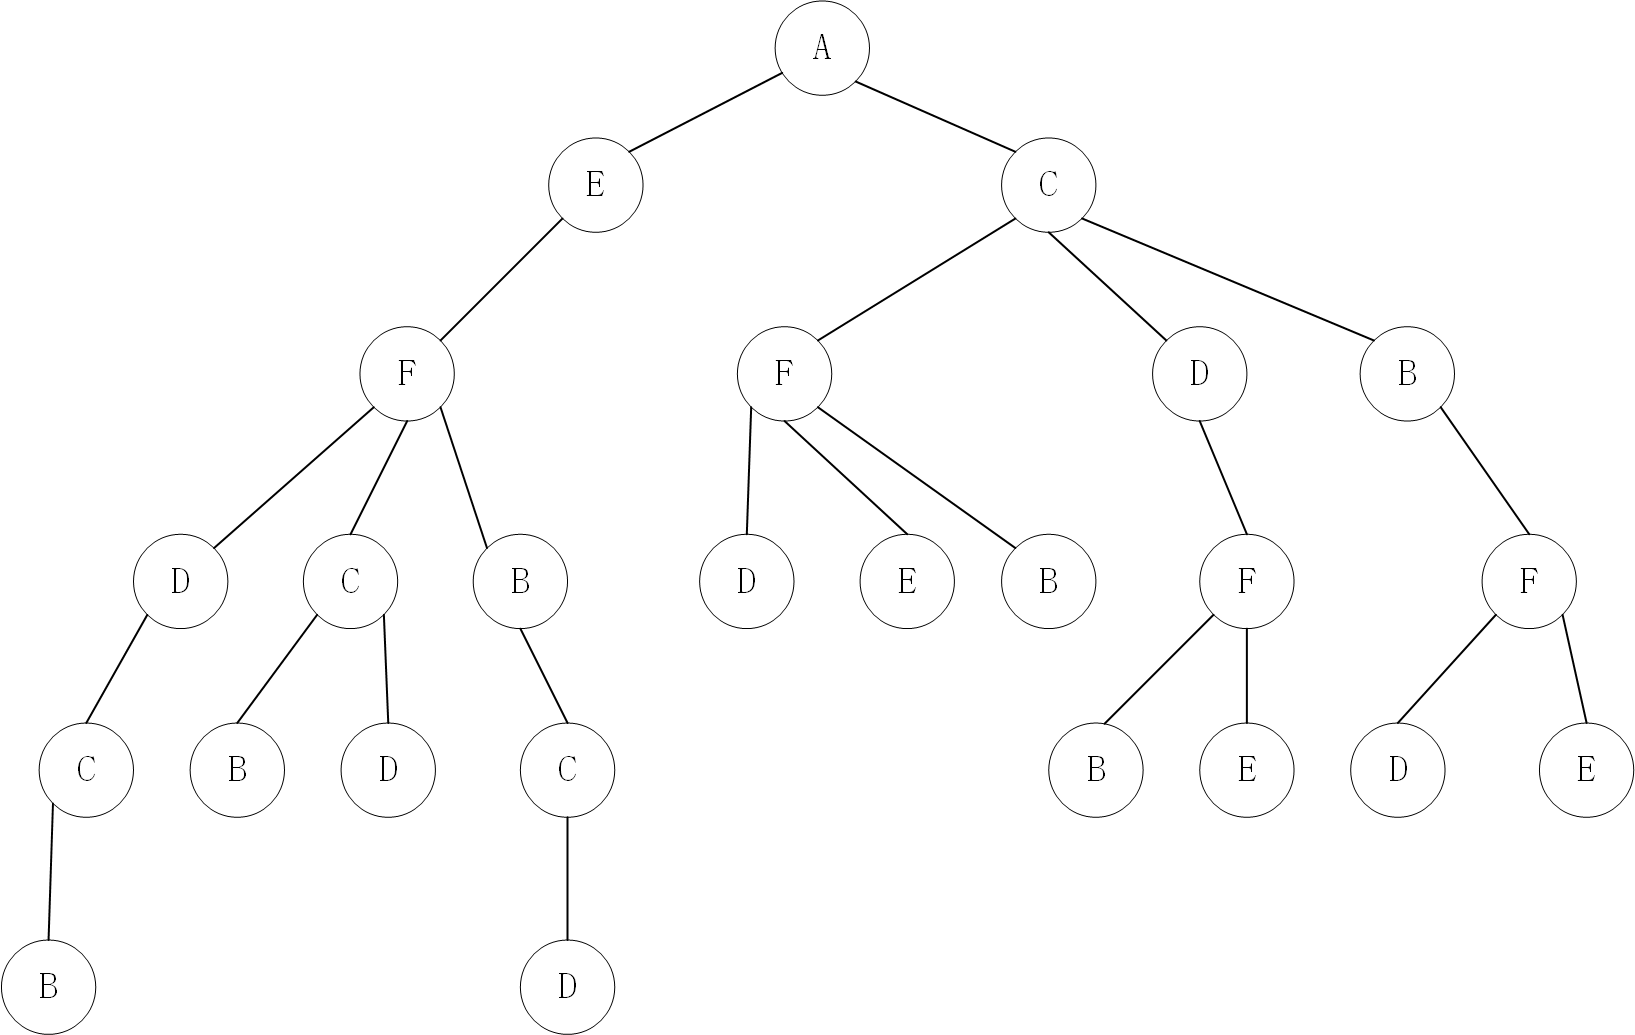
\includegraphics[scale=0.6]{Q1_visual_Tree.png}
	\caption{expanding tree stricture}
	\label{fig:label}
\end{figure}

\begin{figure}
	\begin{minipage}[c]{0.4\textwidth} %minipage使之保持同一行,0.2占这行的0.2
		\centering
		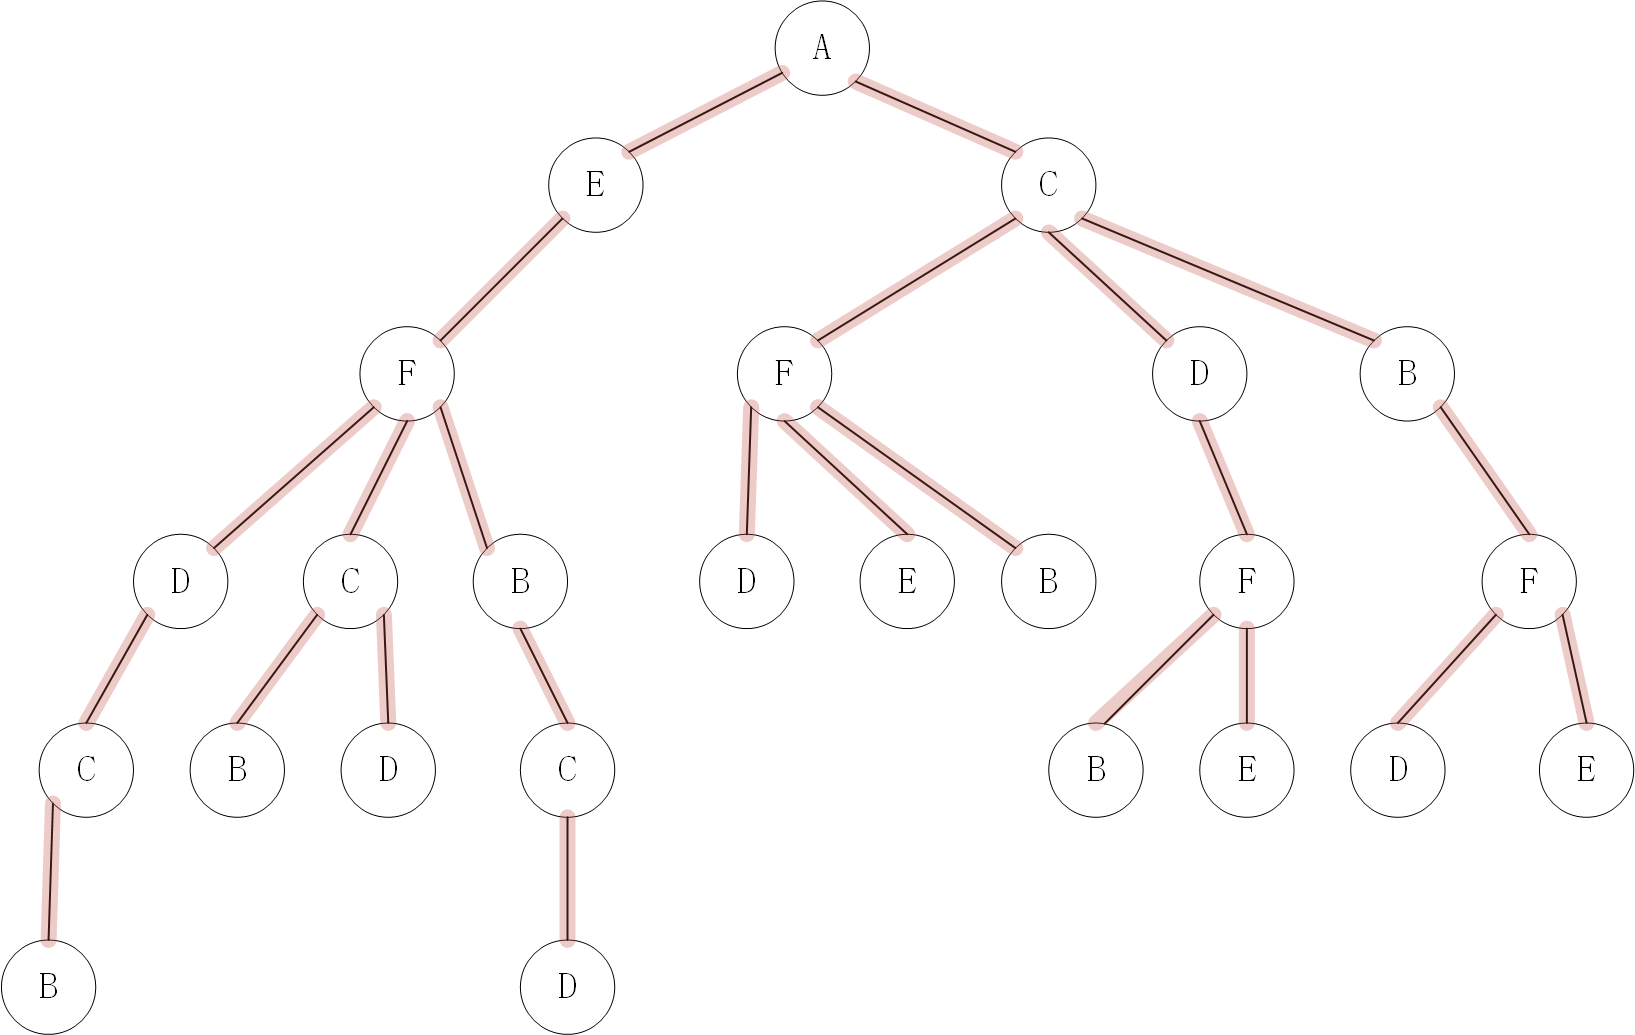
\includegraphics[width=0.7\textwidth]{Q1_visual_DFS.png} %0.5指图片宽度
		\caption{depth-first search algorithm}
	\end{minipage}%
	\begin{minipage}[c]{0.4\textwidth} %minipage使之保持同一行,0.2占这行的0.2
		\centering
		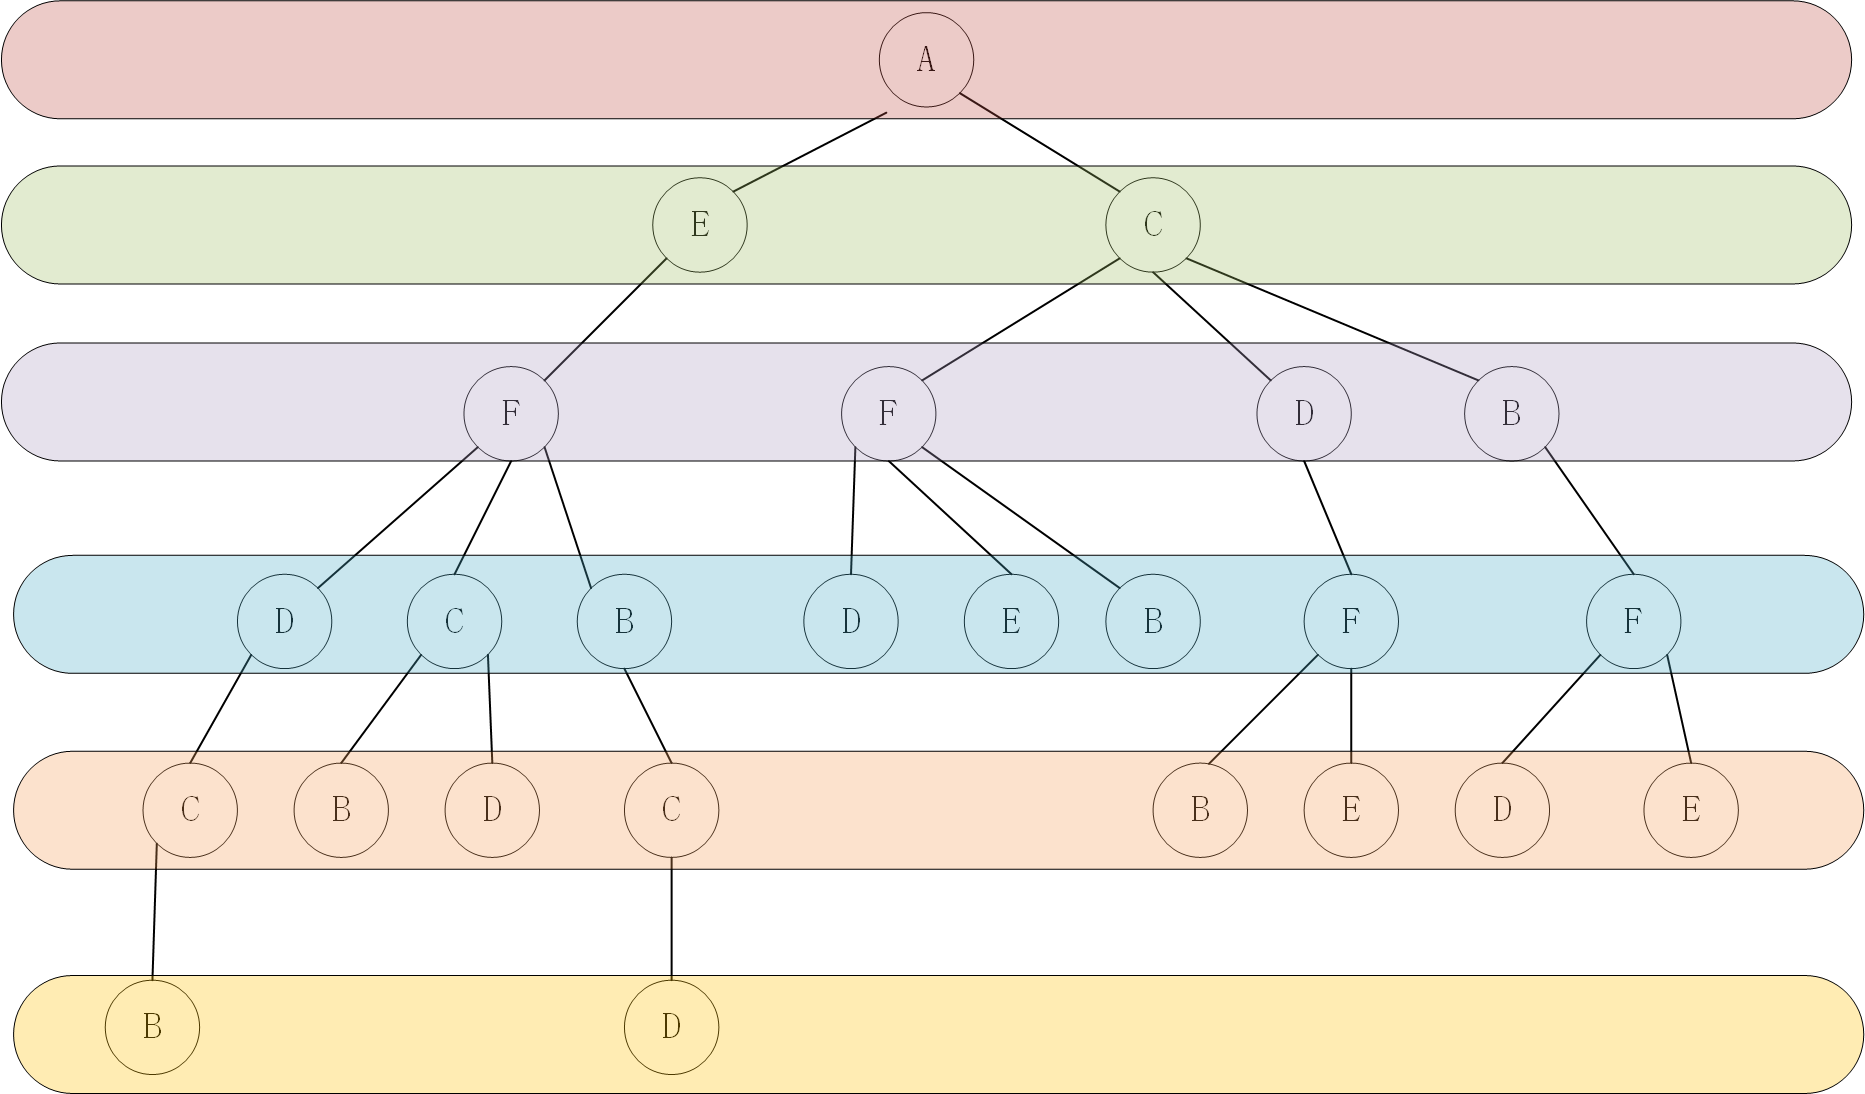
\includegraphics[width=0.7\textwidth]{Q1_visual_BFS.png} %0.5指图片宽度
		\caption{breadth-first search algorithm}
	\end{minipage}%

\end{figure}

\begin{figure}
	\begin{minipage}[c]{0.4\textwidth} %minipage使之保持同一行,0.2占这行的0.2
		\centering
		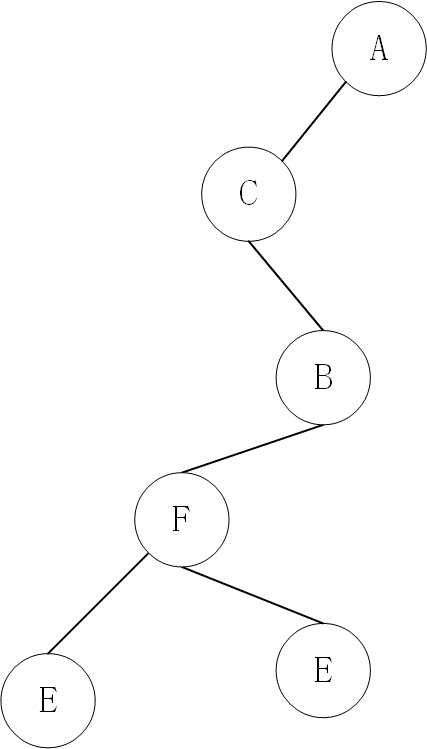
\includegraphics[width=0.7\textwidth]{Q1_visual_DFS_Tree.png} %0.5指图片宽度
		\caption{depth-first search tree}
	\end{minipage}%
	\begin{minipage}[c]{0.4\textwidth} %minipage使之保持同一行,0.2占这行的0.2
		\centering
		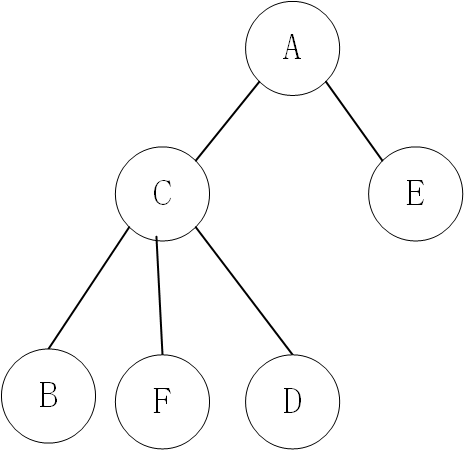
\includegraphics[width=0.7\textwidth]{Q1_visual_BFS_Tree.png} %0.5指图片宽度
		\caption{breadth-first search tree}
	\end{minipage}%

\end{figure}


\textbf{Question: If the graph has \emph{n} nodes and the maximum degree for each node is \emph{d}, what is the complexity of BFS and DFS?}

If the graph has \emph{n} nodes and the maximum degree for each node is \emph{d}, the time complexity of BFS and DFS is both $ O(nd) $. And 
the space complexity of BFS and DFS is both $ O(n) $.


\newpage

\subsubsection{Problem 2}
\begin{itemize}
	\item Step 1: 
				\begin{itemize}
					\item Expand: A
					\item Fringe List: A-C(3), A-B(10), A-D(20)
					\item Closed Set: A
				\end{itemize}
	\item Step 2: 
		 		\begin{itemize}
					\item Expand: A-C
					\item Fringe List: A-C-B(5), A-B(10), A-C-E(18), A-D(20)
					\item Closed Set: A, A-C
				\end{itemize}
	\item Step 3: 
				\begin{itemize}
				   \item Expand: A-C-B
				   \item Fringe List: A-C-B-D(10), A-B(10), A-C-E(18), A-D(20)
				   \item Closed Set: A, A-C, A-C-B
			   \end{itemize}
	\item Step 4: 
			   \begin{itemize}
				  \item Expand: A-C-B-D
				  \item Fringe List: A-C-B-D-E(21), A-B(10), A-C-E(18), A-D(20)
				  \item Closed Set: A, A-C, A-C-B, A-C-B-D
			  \end{itemize}

	\item and we can obtain the shortest path A-C-B-D-E, which lenth is 21 from A to E.
\end{itemize}



\subsubsection{Problem 3}
As the heuristic \emph{h} is admissible if $ 0\leq h(n)\leq h^*(n) $. The \emph{Manhattan distance} is chosen as heuristic \emph{h}.
For the grid $(x,y)$, \emph{h} is given by:

$$ h(n)=|x-5|+|y-2|$$
FIG. shows the value of $ h(n) $ of each grid and the value of $ g(n) $ of each grid. 
To determine the path finding process, I write the code \emph{Q3} which uses A* algorithm. The code is included in its entirety in Appendix.
With the help of A* algorithm, the route is chosen by:

\begin{figure}
	\centering
	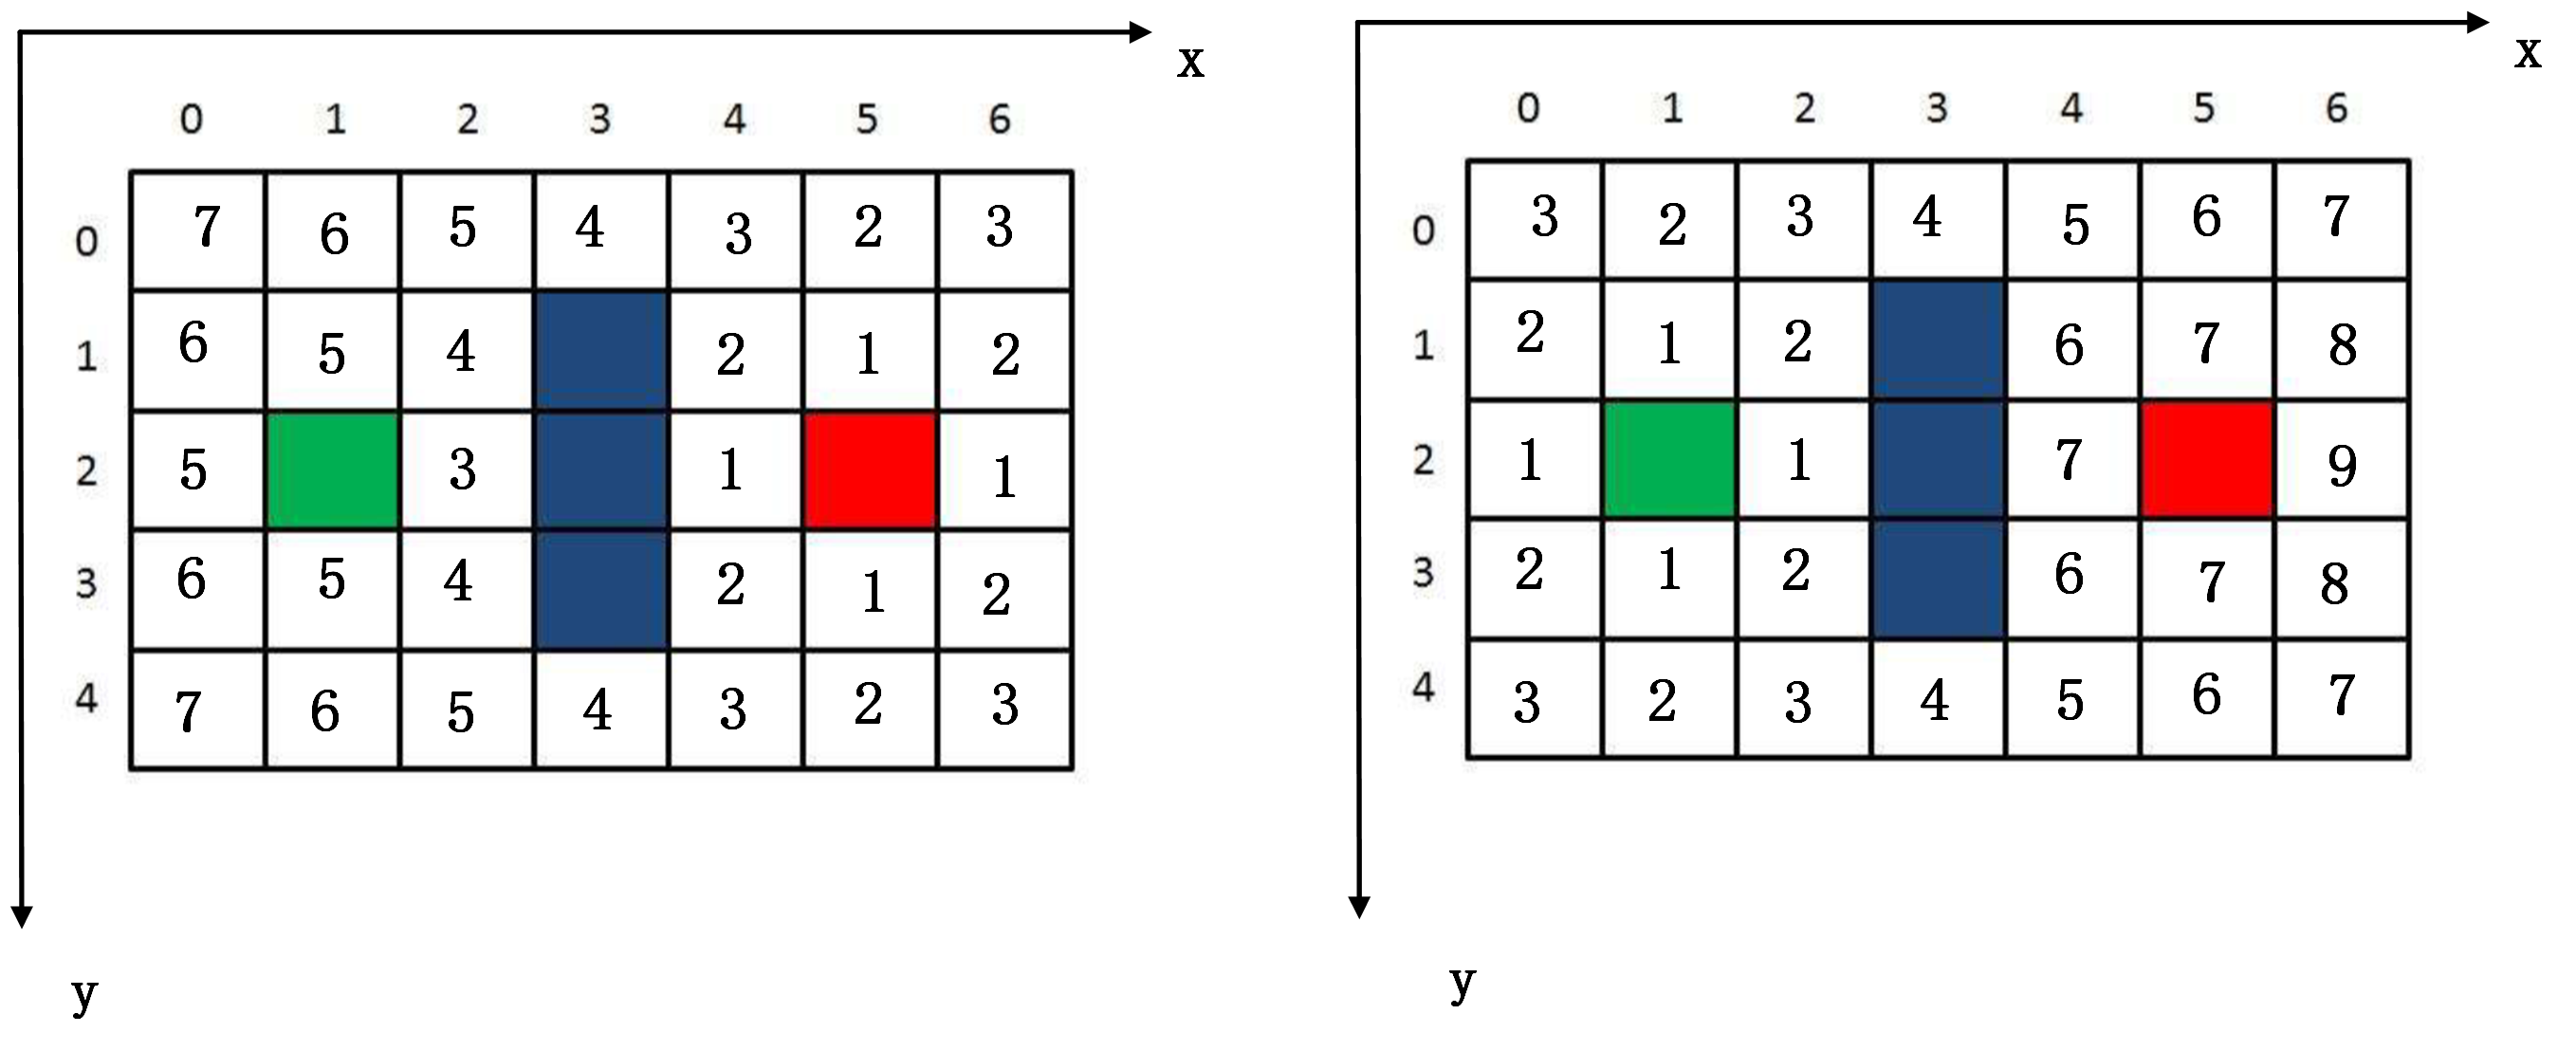
\includegraphics[scale=0.5]{Astar_h&g.png}
	\caption{the value of $ h(n) $ and $g(n)$ of each grid}
	\label{fig:label}
\end{figure}

\begin{figure}
	\centering
	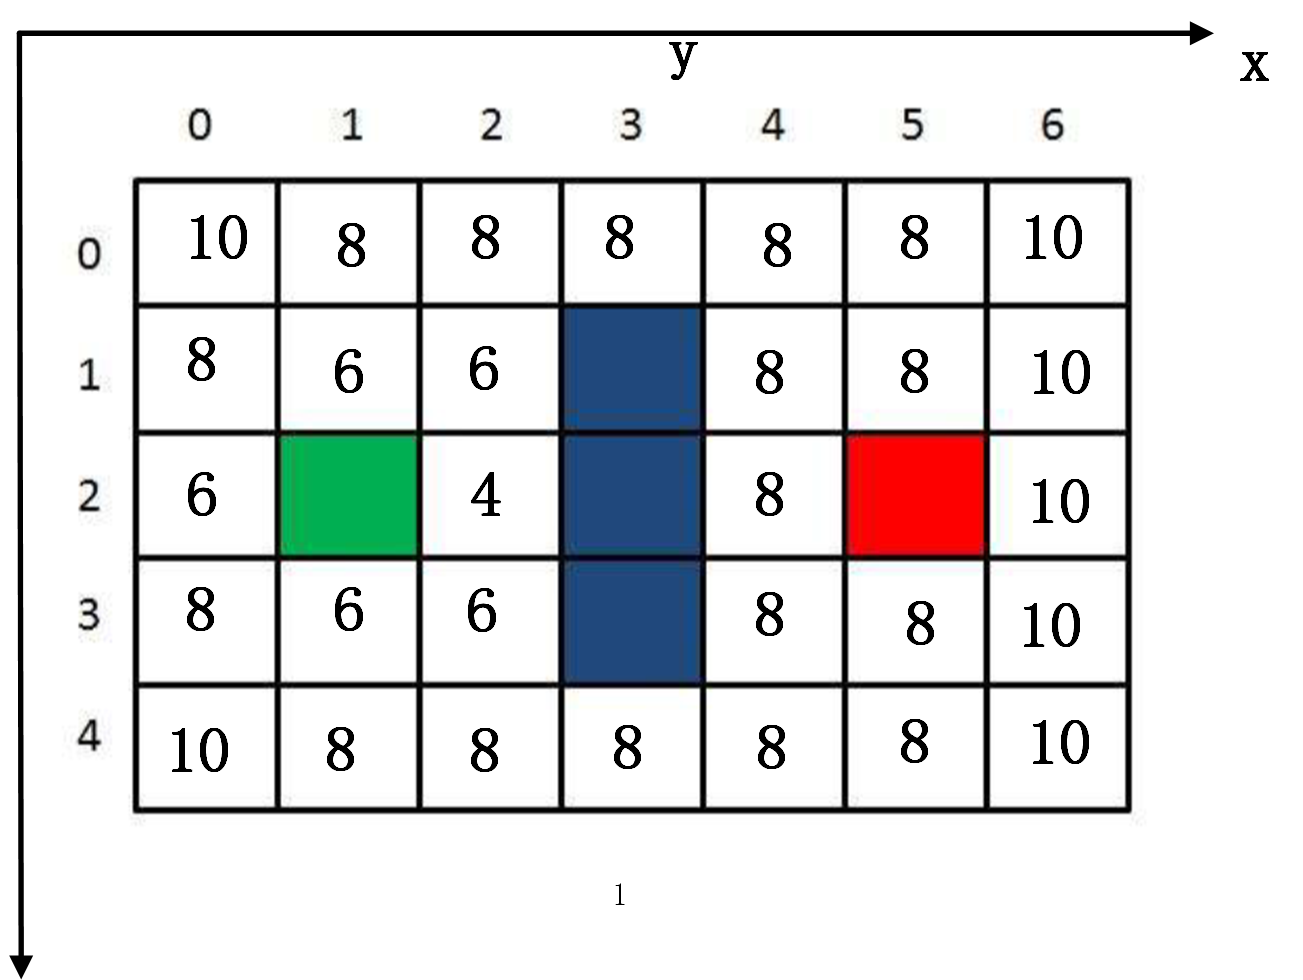
\includegraphics[scale=0.5]{Astar_f.png}
	\caption{the value of $ f(n) $ of each grid}
	\label{fig:label}
\end{figure}


\begin{itemize}
	\item step 1
[1, 2]


fringe list
[(4, [[1, 2], [2, 2], 1]), (6, [[1, 2], [0, 2], 1]), (6, [[1, 2], [1, 3], 1]), (6, [[1, 2], [1, 1], 1])]


closed set
[[1, 2], [1, 2]]


\item step 2
[2, 2]


fringe list
[(6, [[1, 2], [0, 2], 1]), (6, [[1, 2], [1, 1], 1]), (6, [[1, 2], [1, 3], 1]), (6, [[2, 2], [2, 1], 2]), (6, [[2, 2], [2, 3], 2])]


closed set
[[1, 2], [1, 2], [2, 2]]


\item step 3
[0, 2]


fringe list
[(6, [[1, 2], [1, 1], 1]), (6, [[2, 2], [2, 1], 2]), (6, [[1, 2], [1, 3], 1]), (6, [[2, 2], [2, 3], 2]), (8, [[0, 2], [0, 1], 2]), (8, [[0, 2], [0, 3], 2])]


closed set
[[1, 2], [1, 2], [2, 2], [0, 2]]


\item step 4
[1, 1]


fringe list
[(6, [[1, 1], [2, 1], 2]), (6, [[1, 2], [1, 3], 1]), (8, [[0, 2], [0, 3], 2]), (6, [[2, 2], [2, 1], 2]), (8, [[0, 2], [0, 1], 2]), (8, [[1, 1], [0, 1], 2]), (8, [[1, 1], 
[1, 0], 2]), (6, [[2, 2], [2, 3], 2])]


closed set
[[1, 2], [1, 2], [2, 2], [0, 2], [1, 1]]


\item step 5
[2, 1]


fringe list
[(6, [[1, 2], [1, 3], 1]), (6, [[2, 2], [2, 1], 2]), (8, [[0, 2], [0, 3], 2]), (6, [[2, 2], [2, 3], 2]), (8, [[0, 2], [0, 1], 2]), (8, [[1, 1], [0, 1], 2]), (8, [[1, 1], 
[1, 0], 2]), (8, [[2, 1], [2, 0], 3])]


closed set
[[1, 2], [1, 2], [2, 2], [0, 2], [1, 1], [2, 1]]


\item step 6
[1, 3]


fringe list
[(6, [[1, 3], [2, 3], 2]), (6, [[2, 2], [2, 1], 2]), (8, [[0, 2], [0, 3], 2]), (8, [[1, 3], [0, 3], 2]), (6, [[2, 2], [2, 3], 2]), (8, [[1, 1], [0, 1], 2]), (8, [[1, 1], 
[1, 0], 2]), (8, [[2, 1], [2, 0], 3]), (8, [[1, 3], [1, 4], 2]), (8, [[0, 2], [0, 1], 2])]


closed set
[[1, 2], [1, 2], [2, 2], [0, 2], [1, 1], [2, 1], [1, 3]]


\item step 7
[2, 3]


fringe list
[(6, [[2, 2], [2, 1], 2]), (6, [[2, 2], [2, 3], 2]), (8, [[0, 2], [0, 3], 2]), (8, [[1, 3], [0, 3], 2]), (8, [[0, 2], [0, 1], 2]), (8, [[1, 1], [0, 1], 2]), (8, [[1, 1], 
[1, 0], 2]), (8, [[2, 1], [2, 0], 3]), (8, [[1, 3], [1, 4], 2]), (8, [[2, 3], [2, 4], 3])]


closed set
[[1, 2], [1, 2], [2, 2], [0, 2], [1, 1], [2, 1], [1, 3], [2, 3]]


\item step 8
[0, 1]


fringe list
[(8, [[0, 2], [0, 3], 2]), (8, [[1, 3], [0, 3], 2]), (8, [[1, 1], [0, 1], 2]), (8, [[1, 3], [1, 4], 2]), (8, [[2, 3], [2, 4], 3]), (8, [[2, 1], [2, 0], 3]), (8, [[1, 1], 
[1, 0], 2]), (10, [[0, 1], [0, 0], 3])]


closed set
[[1, 2], [1, 2], [2, 2], [0, 2], [1, 1], [2, 1], [1, 3], [2, 3], [0, 1]]


\item step 9
[0, 3]


fringe list
[(8, [[1, 1], [0, 1], 2]), (8, [[1, 3], [0, 3], 2]), (8, [[1, 1], [1, 0], 2]), (8, [[1, 3], [1, 4], 2]), (8, [[2, 3], [2, 4], 3]), (8, [[2, 1], [2, 0], 3]), (10, [[0, 1], [0, 0], 3]), (10, [[0, 3], [0, 4], 3])]


closed set
[[1, 2], [1, 2], [2, 2], [0, 2], [1, 1], [2, 1], [1, 3], [2, 3], [0, 1], [0, 3]]


\item step 10
[1, 0]


fringe list
[(8, [[1, 0], [2, 0], 3]), (8, [[1, 3], [0, 3], 2]), (8, [[2, 1], [2, 0], 3]), (8, [[1, 3], [1, 4], 2]), (8, [[2, 3], [2, 4], 3]), (10, [[0, 3], [0, 4], 3]), (10, [[1, 0], [0, 0], 3]), (10, [[0, 1], [0, 0], 3])]


closed set
[[1, 2], [1, 2], [2, 2], [0, 2], [1, 1], [2, 1], [1, 3], [2, 3], [0, 1], [0, 3], [1, 0]]


\item step 11
[2, 0]


fringe list
[(8, [[1, 3], [0, 3], 2]), (8, [[1, 3], [1, 4], 2]), (8, [[2, 1], [2, 0], 3]), (8, [[2, 0], [3, 0], 4]), (8, [[2, 3], [2, 4], 3]), (10, [[0, 3], [0, 4], 3]), (10, [[1, 0], [0, 0], 3]), (10, [[0, 1], [0, 0], 3])]


closed set
[[1, 2], [1, 2], [2, 2], [0, 2], [1, 1], [2, 1], [1, 3], [2, 3], [0, 1], [0, 3], [1, 0], [2, 0]]


\item step 12
[1, 4]


fringe list
[(8, [[1, 4], [2, 4], 3]), (8, [[2, 0], [3, 0], 4]), (8, [[2, 1], [2, 0], 3]), (8, [[2, 3], [2, 4], 3]), (10, [[1, 0], [0, 0], 3]), (10, [[0, 3], [0, 4], 3]), (10, [[1, 4], [0, 4], 3]), (10, [[0, 1], [0, 0], 3])]


closed set
[[1, 2], [1, 2], [2, 2], [0, 2], [1, 1], [2, 1], [1, 3], [2, 3], [0, 1], [0, 3], [1, 0], [2, 0], [1, 4]]


\item step 13
[2, 4]


fringe list
[(8, [[2, 0], [3, 0], 4]), (8, [[2, 3], [2, 4], 3]), (8, [[2, 1], [2, 0], 3]), (8, [[2, 4], [3, 4], 4]), (10, [[1, 0], [0, 0], 3]), (10, [[0, 3], [0, 4], 3]), (10, [[1, 4], [0, 4], 3]), (10, [[0, 1], [0, 0], 3])]


closed set
[[1, 2], [1, 2], [2, 2], [0, 2], [1, 1], [2, 1], [1, 3], [2, 3], [0, 1], [0, 3], [1, 0], [2, 0], [1, 4], [2, 4]]


\item step 14
[3, 0]


fringe list
[(8, [[2, 1], [2, 0], 3]), (8, [[2, 3], [2, 4], 3]), (10, [[0, 1], [0, 0], 3]), (8, [[2, 4], [3, 4], 4]), (10, [[1, 0], [0, 0], 3]), (10, [[0, 3], [0, 4], 3]), (10, [[1, 
4], [0, 4], 3]), (8, [[3, 0], [4, 0], 5])]


closed set
[[1, 2], [1, 2], [2, 2], [0, 2], [1, 1], [2, 1], [1, 3], [2, 3], [0, 1], [0, 3], [1, 0], [2, 0], [1, 4], [2, 4], [3, 0]]


\item step 15
[3, 4]


fringe list
[(8, [[3, 0], [4, 0], 5]), (10, [[0, 3], [0, 4], 3]), (8, [[3, 4], [4, 4], 5]), (10, [[1, 4], [0, 4], 3]), (10, [[1, 0], [0, 0], 3]), (10, [[0, 1], [0, 0], 3])]


closed set
[[1, 2], [1, 2], [2, 2], [0, 2], [1, 1], [2, 1], [1, 3], [2, 3], [0, 1], [0, 3], [1, 0], [2, 0], [1, 4], [2, 4], [3, 0], [3, 4]]


\item step 16
[4, 0]


fringe list
[(8, [[3, 4], [4, 4], 5]), (10, [[0, 3], [0, 4], 3]), (8, [[4, 0], [4, 1], 6]), (10, [[1, 4], [0, 4], 3]), (10, [[1, 0], [0, 0], 3]), (10, [[0, 1], [0, 0], 3]), (8, [[4, 
0], [5, 0], 6])]


closed set
[[1, 2], [1, 2], [2, 2], [0, 2], [1, 1], [2, 1], [1, 3], [2, 3], [0, 1], [0, 3], [1, 0], [2, 0], [1, 4], [2, 4], [3, 0], [3, 4], [4, 0]]


\item step 17
[4, 4]


fringe list
[(8, [[4, 0], [4, 1], 6]), (8, [[4, 4], [5, 4], 6]), (8, [[4, 0], [5, 0], 6]), (10, [[0, 3], [0, 4], 3]), (10, [[1, 0], [0, 0], 3]), (10, [[0, 1], [0, 0], 3]), (8, [[4, 4], [4, 3], 6]), (10, [[1, 4], [0, 4], 3])]


closed set
[[1, 2], [1, 2], [2, 2], [0, 2], [1, 1], [2, 1], [1, 3], [2, 3], [0, 1], [0, 3], [1, 0], [2, 0], [1, 4], [2, 4], [3, 0], [3, 4], [4, 0], [4, 4]]


\item step 18
[4, 1]


fringe list
[(8, [[4, 0], [5, 0], 6]), (8, [[4, 1], [4, 2], 7]), (8, [[4, 4], [4, 3], 6]), (8, [[4, 1], [5, 1], 7]), (10, [[1, 0], [0, 0], 3]), (10, [[0, 1], [0, 0], 3]), (10, [[1, 4], [0, 4], 3]), (10, [[0, 3], [0, 4], 3]), (8, [[4, 4], [5, 4], 6])]


closed set
[[1, 2], [1, 2], [2, 2], [0, 2], [1, 1], [2, 1], [1, 3], [2, 3], [0, 1], [0, 3], [1, 0], [2, 0], [1, 4], [2, 4], [3, 0], [3, 4], [4, 0], [4, 4], [4, 1]]


\item step 19
[5, 0]


fringe list
[(8, [[4, 1], [4, 2], 7]), (8, [[4, 1], [5, 1], 7]), (8, [[4, 4], [4, 3], 6]), (8, [[4, 4], [5, 4], 6]), (10, [[1, 0], [0, 0], 3]), (10, [[0, 1], [0, 0], 3]), (10, [[1, 4], [0, 4], 3]), (10, [[0, 3], [0, 4], 3]), (8, [[5, 0], [5, 1], 7]), (10, [[5, 0], [6, 0], 7])]


closed set
[[1, 2], [1, 2], [2, 2], [0, 2], [1, 1], [2, 1], [1, 3], [2, 3], [0, 1], [0, 3], [1, 0], [2, 0], [1, 4], [2, 4], [3, 0], [3, 4], [4, 0], [4, 4], [4, 1], [5, 0]]


\item step 20
[4, 2]


fringe list
[(8, [[4, 1], [5, 1], 7]), (8, [[4, 2], [5, 2], 8]), (8, [[4, 4], [4, 3], 6]), (8, [[5, 0], [5, 1], 7]), (8, [[4, 4], [5, 4], 6]), (10, [[0, 1], [0, 0], 3]), (10, [[1, 4], [0, 4], 3]), (10, [[0, 3], [0, 4], 3]), (10, [[5, 0], [6, 0], 7]), (10, [[4, 2], [4, 3], 8]), (10, [[1, 0], [0, 0], 3])]


closed set
[[1, 2], [1, 2], [2, 2], [0, 2], [1, 1], [2, 1], [1, 3], [2, 3], [0, 1], [0, 3], [1, 0], [2, 0], [1, 4], [2, 4], [3, 0], [3, 4], [4, 0], [4, 4], [4, 1], [5, 0], [4, 2]]  


\item step 21
[5, 1]


fringe list
[(8, [[4, 2], [5, 2], 8]), (8, [[4, 4], [5, 4], 6]), (8, [[4, 4], [4, 3], 6]), (8, [[5, 0], [5, 1], 7]), (8, [[5, 1], [5, 2], 8]), (10, [[0, 1], [0, 0], 3]), (10, [[1, 4], [0, 4], 3]), (10, [[0, 3], [0, 4], 3]), (10, [[5, 0], [6, 0], 7]), (10, [[4, 2], [4, 3], 8]), (10, [[1, 0], [0, 0], 3]), (10, [[5, 1], [6, 1], 8])]


closed set
[[1, 2], [1, 2], [2, 2], [0, 2], [1, 1], [2, 1], [1, 3], [2, 3], [0, 1], [0, 3], [1, 0], [2, 0], [1, 4], [2, 4], [3, 0], [3, 4], [4, 0], [4, 4], [4, 1], [5, 0], [4, 2], [5, 1]]


\item step 22
[5, 2]


final path
['(1,2)', '(1,1)', '(1,0)', '(2,0)', '(3,0)', '(4,0)', '(4,1)', '(4,2)', '(5,2)']
\end{itemize}

\subsubsection{Problem 4}

\begin{itemize}
	\item \emph{BFSvsDFS.py}

	The file provides the class \emph{Graph}, which includes a dictionary \emph{edges} and function \emph{neighbors}.  
	\emph{edges} is treated as dictionary to look up. 
	Function \emph{neighbors} pass in an id and returns a list of neighboring node

	\begin{itemize}
		\item function \emph{reconstruct\underline{ }path(came\underline{ }from, start, goal)}
		
		Given a dictionary named \emph{came\underline{ }from}. The key of the dictionary is the node 
    	character and its value is the parent node, the start node
		and the goal node, the function will compute the path from start to the end.


		\vspace{3mm}
		To accomplish this function, I start with \emph{goal} because each node might have more than one children 
		but one father node only. With the \emph{came\underline{ }from} provided, I can search for the father node of every node.
		Start with \emph{goal} and append its father to the \emph{path} list. Loop untill \emph{start} appears as a node's father.
		At last, reverse the list and return it as result.

		\begin{lstlisting}
			def reconstruct_path(came_from, start, goal):
				path = []
				### START CODE HERE ### (≈ 6 line of code)
				if came_from is None:
					print("Path reconstruction failed!!")
					return 

				current_node = goal
				while(current_node is not start):
					path.append(current_node)
					current_node = came_from[current_node]
				path.append(current_node)
				path.reverse()

				### END CODE HERE ###
				return path
			
		\end{lstlisting}
		\vspace{3mm}
		%==========================================================================
		\item function \emph{breadth\underline{ }first\underline{ }search(graph, start, goal)}
		
		Given a graph, a start node and a goal node, 
    	the function utilizes breadth first search algorithm to find the path from 
    	start node to the goal node. It will return a dictionary whose key is each node and corresponding  
		value is its parent node
		\vspace{3mm}

		To accomplish this function, I use \emph{queue} to expand the search region. The elements in the queue are stored as format \emph{[father, child]}.
		Firstly put the \emph{[None, start]} into the queue, While the queue is not empty, get the element from the head of queue as variable \emph{Expand}.
		Add the father and child of \emph{Expand} into the \emph{came\underline{ }from} dictionary. 
		To realize \textbf{early stoping} mentioned in the code, I check if \emph{goal} neighbors to the child of \emph{Expand}. If so, add the goal to the dictionary as
		child of child in \emph{Expand}, then return \emph{came\underline{ }from}.
		

		\vspace{3mm}
		It needs to be aware that for a gragh search, you should never expand a state twice. So I set the list \emph{closed\underline{ }set} to store the node that has been put into the queue.
		Before putting any node into the queue, check the node if it is in the \emph{closed\underline{ }set}.
		
		\begin{lstlisting}
			def breadth_first_search(graph, start, goal):
				came_from = {}
				came_from[start] = None
				### START CODE HERE ### (≈ 10 line of code)

				## check goal and start ===========================
				if not ((goal in graph.edges) and (start in graph.edges) ):
					print("Error! Goal or Start is not in the graph")
					return None
				##=================================================
				
				closed_set = [start]
				BFS_queue = Queue(maxsize=0)
				BFS_queue.put([None, start])
				while not BFS_queue.empty():
					Expand = BFS_queue.get()
					came_from[Expand[1]] = Expand[0]
					if goal in graph.neighbors(Expand[1]):
						came_from[goal] = Expand[1]
						return came_from
					for value in graph.neighbors(Expand[1]):
						if value not in closed_set:
							BFS_queue.put([Expand[1], value])
							closed_set.append(value)

				### END CODE HERE ###
    			return came_from
		\end{lstlisting}
		\vspace{3mm}
		%==========================================================================

		\item function \emph{depth\underline{ }first\underline{ }search(graph, start, goal)}
		
		Given a graph, a start node and a goal node, 
    	the function utilizes depth first search algorithm to find the path from 
    	start node to the goal node. It will return a dictionary whose key is each node and corresponding  
		value is its parent node
		\vspace{3mm}

		To accomplish this function, I use \emph{stack} to expand the search region. The elements in the stack are stored as format \emph{[father, child]}.
		Firstly put the \emph{[None, start]} into the stack, While the stack is not empty, get the element from the head of stack as variable \emph{Expand}.
		Add the father and child of \emph{Expand} into the \emph{came\underline{ }from} dictionary. 
		To realize \textbf{early stoping} mentioned in the code, I check if \emph{goal} neighbors to the child of \emph{Expand}. If so, add the goal to the dictionary as
		child of child in \emph{Expand}, then return \emph{came\underline{ }from}.
		
		\vspace{3mm}
		It needs to be aware that for a gragh search, you should never expand a state twice. So I set the list \emph{closed\underline{ }set} to store the node that has been put into the stack.
		Before putting any node into the stack, check the node if it is in the \emph{closed\underline{ }set}.

		\begin{lstlisting}
			def depth_first_search(graph, start, goal):
				came_from = {}
				came_from[start] = None
				### START CODE HERE ### (≈ 10 line of code)

				## check goal and start ===========================
				if not ((goal in graph.edges) and (start in graph.edges) ):
					print("Error! Goal or Start is not in the graph")
					return 
				##=================================================

				closed_set = [start]
				DFS_queue = LifoQueue(maxsize=0)
				DFS_queue.put([None, start])
				while not DFS_queue.empty():
					Expand = DFS_queue.get()
					came_from[Expand[1]] = Expand[0]
					if goal in graph.neighbors(Expand[1]):
						came_from[goal] = Expand[1]
						return came_from
					for value in graph.neighbors(Expand[1]):
						if value not in closed_set:
							DFS_queue.put([Expand[1], value])
							closed_set.append(value)

				### END CODE HERE ###
				
				return came_from
		\end{lstlisting}
		
	\end{itemize}

	The demonstrations for functions  will be shown in part \textbf{\RNum{2} EXPERIMENT} 
	%----------------------------------------------------------------------------------------------

	\item \emph{UniformCostSearch.py}
	
	The file provides the class \emph{Graph}, which includes the dictionary \emph{edges}, the dictionary \emph{edgeWeights}, the function \emph{neighbors} and the function \emph{get\underline{ }cost}.
	\emph{edges} and \emph{edgeWeights} are treated as dictionary to look up. 
	Pass in an id to function \emph{neighbors}, it will return a list of neighboring node, while \emph{get\underline{ }cost} accepts two adjacent nodes and returns the cost.

	\begin{itemize}
		\item function \emph{reconstruct\underline{ }path(came\underline{ }from, start, goal)}
		
		Given a dictionary named \emph{came\underline{ }from}. The key of dictionary is the node 
    	character and its value is the parent node, the start node
		and the goal node, the function will compute the path from start to the end.


		\vspace{3mm}
		To accomplish this function, I start with \emph{goal} because each node might have more than one children 
		but one father node only. With the \emph{came\underline{ }from} provided, I can search for the father node of every node.
		Start with \emph{goal} and append its father to the \emph{path} list. Loop untill \emph{start} appears as a node's father.
		At last, reverse the list and return it as result.

		\begin{lstlisting}
			def reconstruct_path(came_from, start, goal):
				path = []
				### START CODE HERE ### (≈ 6 line of code)
				if came_from is None:
					print("Path reconstruction failed!!")
					return 

				current_node = goal
				while(current_node is not start):
					path.append(current_node)
					current_node = came_from[current_node]
				path.append(current_node)
				path.reverse()

				### END CODE HERE ###
				return path
			
		\end{lstlisting}
		\vspace{3mm}
		%==========================================================================

		\item function \emph{uniform\underline{ }cost\underline{ }search}
		
		Given a graph, a start node and a goal node, 
    	the function utilizes uniform cost search algorithm to find the path from 
    	start node to the goal node. It will return two dictionaries, whose key is each node and corresponding  
		value is its parent node, and whose key is each node and corresponding value is the cost from start to the node.
		\vspace{3mm}

		To accomplish this function, I use \emph{PriorityQueue} to expand the search region. The elements in the PriorityQueue are stored as format \emph{[value,[father, child]]}.
		Firstly put the \emph{[0,[None, start]]} into the PriorityQueue. While the PriorityQueue is not empty, get the element from the head of PriorityQueue as variable \emph{Expand}.
		Add the father and child of \emph{Expand} into the \emph{came\underline{ }from} dictionary, then add the child and value of \emph{Expand} into the \emph{cost\underline{ }so\underline{ }far}. 
		To realize \textbf{early stoping} mentioned in the code, I check if \emph{goal} neighbors to the child of \emph{Expand}. If so, add the goal to the dictionary as
		child of child in \emph{Expand}, then return \emph{came\underline{ }from} and \emph{cost\underline{ }so\underline{ }far}.
		

		\vspace{3mm}
		It needs to be aware that for a gragh search, you should never expand a state twice. So I set the list \emph{closed\underline{ }set} to store the node that has been put into the PriorityQueue.
		Before putting any node into the PriorityQueue, check the node if it is in the \emph{closed\underline{ }set}.

		\begin{lstlisting}
			def uniform_cost_search(graph, start, goal):
    
				came_from = {}
				cost_so_far = {}
				came_from[start] = None
				cost_so_far[start] = 0
				### START CODE HERE ### (≈ 15 line of code)

				### q.put((num,value)), smaller the num is, higher the priority is
				### the cost_so_far should store the value that the nodes cost from start 
				closed_set = [start]
				UCS_queue = PriorityQueue(maxsize=0)
				UCS_queue.put((0, [None, start]))
				while not UCS_queue.empty():
					### Expand[1][1] is current node, Expand[1][0] is its father
					### Expand[0] is the cost that from start to the Expand[1][1]
					Expand = UCS_queue.get()
					came_from[Expand[1][1]] = Expand[1][0]
					cost_so_far[Expand[1][1]] = Expand[0]
					if goal in graph.neighbors(Expand[1][1]):
						came_from[goal] = Expand[1][1]
						cost_so_far[goal] = graph.get_cost(Expand[1][1], goal) + Expand[0]
						return came_from, cost_so_far
					for value in graph.neighbors(Expand[1][1]):
						if value not in closed_set:
							UCS_queue.put((graph.get_cost(Expand[1][1], value)+Expand[0], [Expand[1][1], value]))
							closed_set.append(value)

				### END CODE HERE ###
				return came_from, cost_so_far
		\end{lstlisting}

		%==========================================================================
	\end{itemize}

	The demonstration for functions will be shown in part \textbf{\RNum{2} EXPERIMENT} 
	%----------------------------------------------------------------------------------------------

	\item \emph{AStarSearch.py}
	
	The file provides the class \emph{Graph}, which includes the dictionary \emph{edges}, the dictionary \emph{edgeWeights}, the function \emph{neighbors} and the function \emph{get\underline{ }cost}.
	\emph{edges} and \emph{edgeWeights} are treated as dictionary to look up. 
	Pass in an id to function \emph{neighbors}, it will return a list of neighboring node, while \emph{get\underline{ }cost} accepts two adjacent nodes and returns the cost.

	\begin{itemize}
		\item function \emph{reconstruct\underline{ }path(came\underline{ }from, start, goal)}
		
		The function is same as the previous \emph{reconstruct\underline{ }path(came\underline{ }from, start, goal)}.

		\item function \emph{def heuristic(graph, current\underline{ }node, goal\underline{ }node)}
		
		I choose \emph{Euclidean distance} between a node and the goal as the heuristic of the node. To check whether the graph satisfies the consistency of heuristics, in the function 
		\emph{heuristic}, I import the function \emph{uniform\underline{ }cost\underline{ }search} to compare the heuristic and the least cost of the node. If the 

		\begin{lstlisting}
			def heuristic(graph, current_node, goal_node):
    
				heuristic_value = 0
				### START CODE HERE ### (≈ 15 line of code)
				
				from UniformCostSearch import uniform_cost_search
				import math

				came_from_UCS, _ = uniform_cost_search(graph, current_node, goal_node)
				path = reconstruct_path(came_from_UCS, current_node, goal)
				
				actural_distance = 0
				for i in range(len(path)-1):
					actural_distance += graph.get_cost(path[i],path[i+1])
				
				heuristic_value = math.sqrt( (graph.locations[current_node][0] - graph.locations[goal_node][0])**2 + (graph.locations[current_node][1] - graph.locations[goal_node][1])**2)
				
				if actural_distance < heuristic_value:
					print("graph doesn't satisfies the consistency of heuristics")

				### END CODE HERE ###
				return heuristic_value
		\end{lstlisting}
		
		If heuristic value is more than actral distance, it means that graph doesn't satisfies the consistency of heuristics

		\item function \emph{A\underline{ }star\underline{ }search}
		
		Given a graph, a start node and a goal node, 
    	the function utilizes A* search algorithm to find the path from 
    	start node to the goal node. It will return two dictionaries, whose key is each node and corresponding  
		value is its parent node, and whose key is each node and corresponding value is the cost from start to the node.
		\vspace{3mm}

		To accomplish this function, I use \emph{PriorityQueue} to expand the search region. The elements in the PriorityQueue are stored as format \emph{[value,[father, child, CostToChild]]}. The \emph{value} computed by adding the cost from start to the current node and the heuristic of the current node. 
		The \emph{CostToChild} is the cost from start to the child node. 
		Firstly put the \emph{[0+heuristic(graph,start,goal), [None, start,0]]} into the PriorityQueue. While the PriorityQueue is not empty, get the element from the head of PriorityQueue as variable \emph{Expand}.
		Add the father and child of \emph{Expand} into the \emph{came\underline{ }from} dictionary, then add the child and CostToChild of \emph{Expand} into the \emph{cost\underline{ }so\underline{ }far}. 
		To realize \textbf{early stoping} mentioned in the code, I check if \emph{goal} neighbors to the child of \emph{Expand}. If so, add the goal to the dictionary as
		child of child in \emph{Expand}, then return \emph{came\underline{ }from} and \emph{cost\underline{ }so\underline{ }far}.

		\begin{lstlisting}
			def A_star_search(graph, start, goal):
				came_from = {}
				cost_so_far = {}
				came_from[start] = None
				cost_so_far[start] = 0

				### START CODE HERE ### (≈ 15 line of code)

				closed_set = set(start)
				Astar_queue = PriorityQueue(maxsize=0)
				Astar_queue.put((0 + heuristic(graph,start,goal), [None, start, 0]))
				while not Astar_queue.empty():
					# Expand[1][1] is current node, Expand[1][0] is its father
					# Expand[0] is the value of h()+g()
					# Expand[1][2] is the cost that from start to the Expand[1][1]
					Expand = Astar_queue.get()
					closed_set.add(Expand[1][1])
					came_from[Expand[1][1]] = Expand[1][0]
					cost_so_far[Expand[1][1]] = Expand[1][2]

					if goal in graph.neighbors(Expand[1][1]):
						came_from[goal] = Expand[1][1]
						cost_so_far[goal] = graph.get_cost(Expand[1][1], goal) + Expand[1][2]
						return came_from, cost_so_far
					for value in graph.neighbors(Expand[1][1]):
						if value not in closed_set:
							Astar_queue.put((graph.get_cost(Expand[1][1], value)+Expand[1][2] + heuristic(graph,value,goal),
																[Expand[1][1], value, graph.get_cost(Expand[1][1], value)+Expand[1][2] ]))
				### END CODE HERE ###
				return came_from, cost_so_far
		\end{lstlisting}
		
		The demonstration for functions will be shown in part \textbf{\RNum{2} EXPERIMENT} 

	\end{itemize} 


\end{itemize}





%%%%%%%%%%%%%%%%%%%%%%%%%%%%%%
%%%%%%%%%%%%%%%%%%%%%%%%%%%%%%
\newpage
\section{Experiment}
This section consists of screenshots taken during the laboratory procedure. 

\subsection{\emph{BFSvsDFS.py}}

For large graph, the search starts from \emph{S} to \emph{E}. For small graph,  the search starts from \emph{A} to \emph{E}.

\begin{figure}[h]
	\begin{minipage}[c]{0.4\textwidth} %minipage使之保持同一行,0.2占这行的0.2
		\centering
		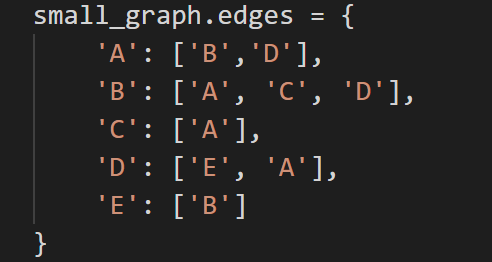
\includegraphics[width=0.7\textwidth]{small_graph.png} %0.5指图片宽度
	\end{minipage}%
	\begin{minipage}[c]{0.4\textwidth} %minipage使之保持同一行,0.2占这行的0.2
		\centering
		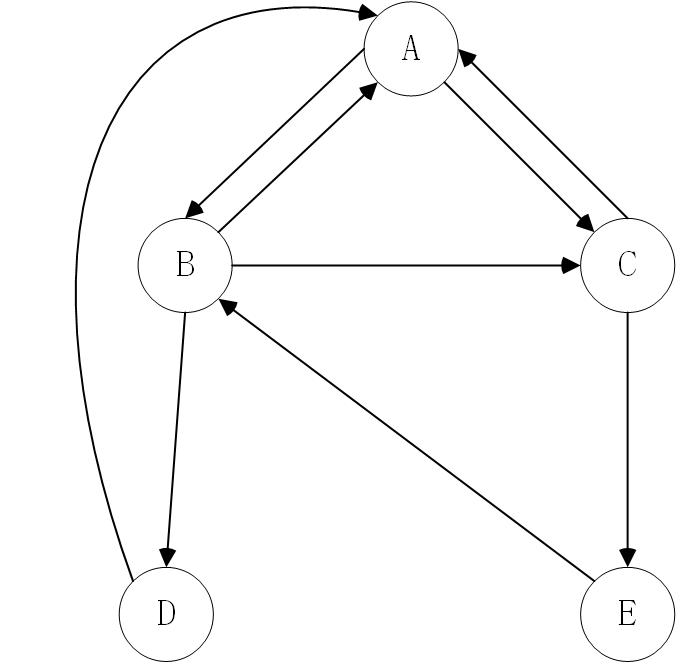
\includegraphics[width=0.7\textwidth]{small_graph_visual.png} %0.5指图片宽度
		
	\end{minipage}%
	\caption{small graph}
\end{figure}

\begin{figure}[h]
	\begin{minipage}[c]{0.4\textwidth} %minipage使之保持同一行,0.2占这行的0.2
		\centering
		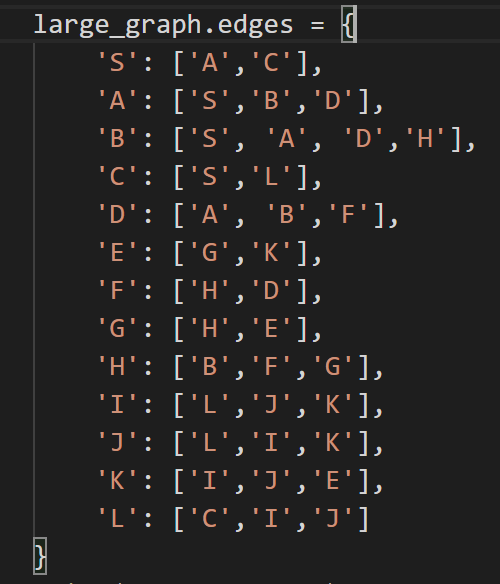
\includegraphics[width=0.8\textwidth]{large_graph.png} %0.5指图片宽度
	\end{minipage}%
	\begin{minipage}[c]{0.4\textwidth} %minipage使之保持同一行,0.2占这行的0.2
		\centering
		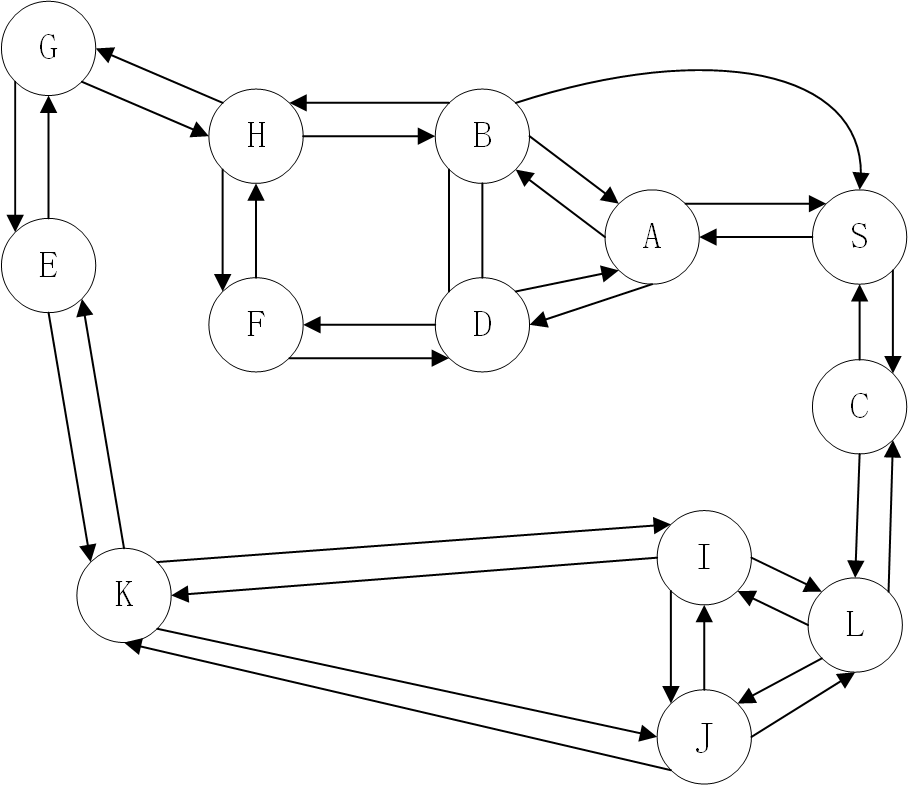
\includegraphics[width=0.8\textwidth]{large_graph_visual.png} %0.5指图片宽度
		
	\end{minipage}%
	\caption{large graph}
\end{figure}

\begin{figure}[h]
	\centering
	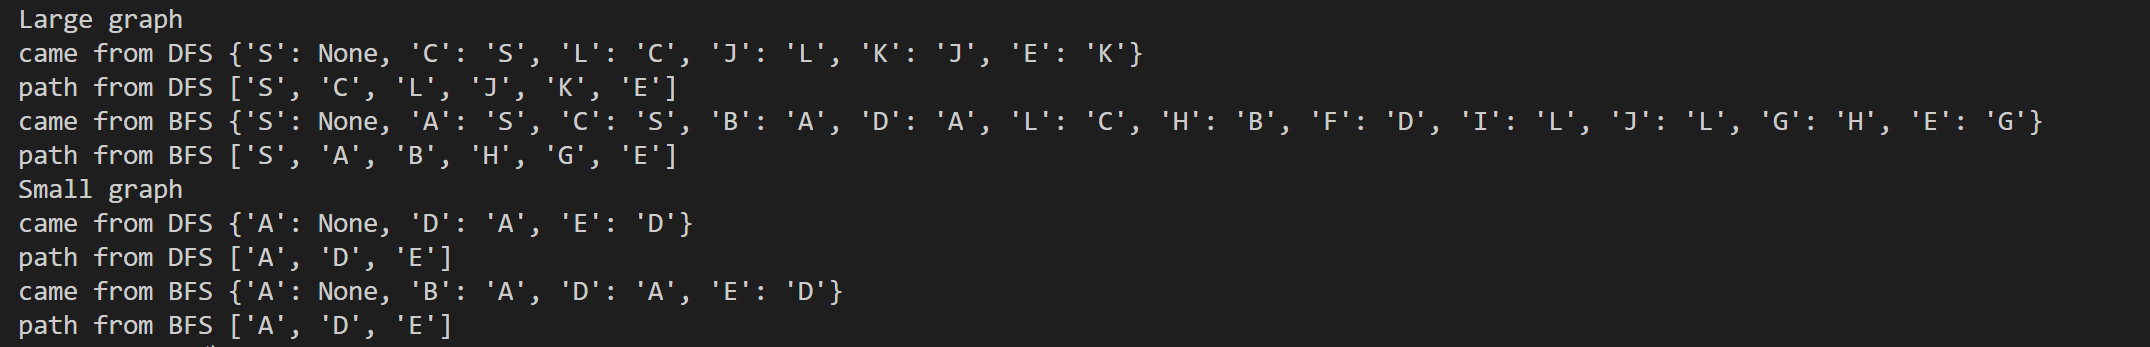
\includegraphics[width=1\textwidth]{BFS_DFS.png}
	\caption{result for BFS and DFS}
	\label{fig:label}
\end{figure}

\subsection{\emph{UniformCostSearch.py}}

For large graph, the search starts from \emph{S} to \emph{H}. For small graph,  the search starts from \emph{A} to \emph{E}.

\begin{figure}[h]
	\begin{minipage}[c]{0.4\textwidth} %minipage使之保持同一行,0.2占这行的0.2
		\centering
		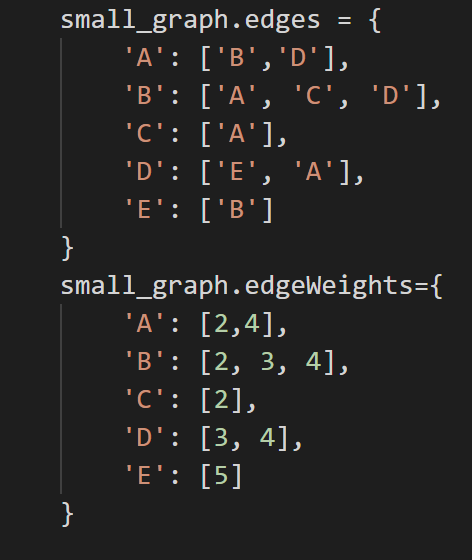
\includegraphics[width=0.7\textwidth]{small_graph_UCS.png} %0.5指图片宽度
	\end{minipage}%
	\begin{minipage}[c]{0.4\textwidth} %minipage使之保持同一行,0.2占这行的0.2
		\centering
		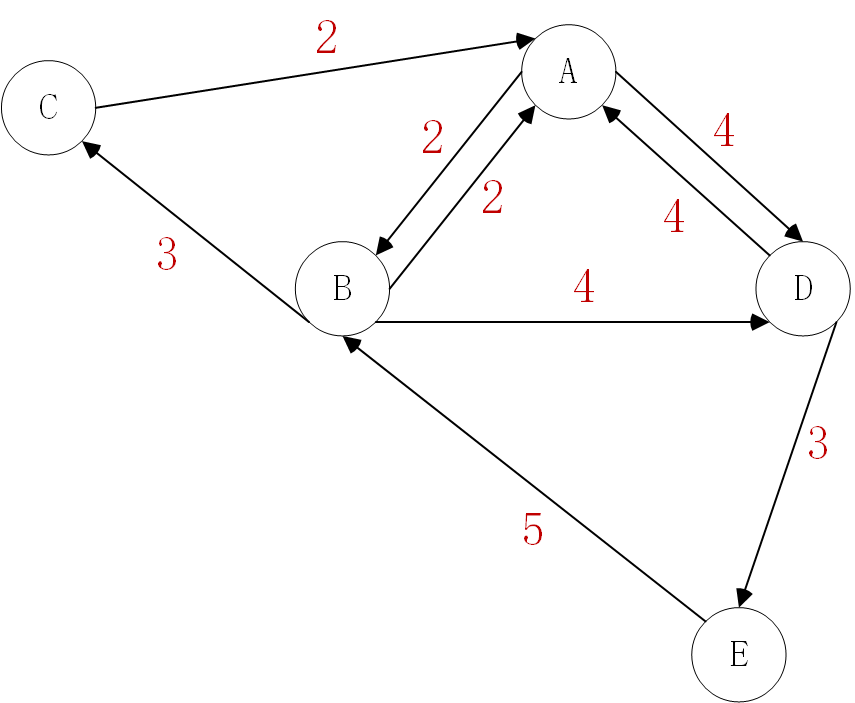
\includegraphics[width=0.7\textwidth]{small_graph_UCS_visual.png} %0.5指图片宽度
		
	\end{minipage}%
	\caption{small graph}
\end{figure}

\begin{figure}[h]
	\begin{minipage}[c]{0.4\textwidth} %minipage使之保持同一行,0.2占这行的0.2
		\centering
		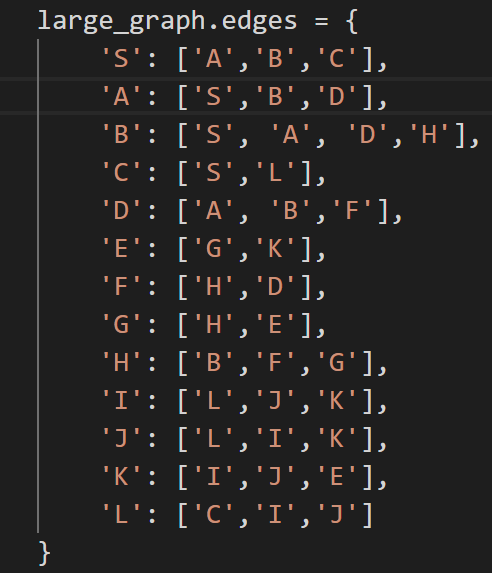
\includegraphics[width=0.8\textwidth]{large_graph_UCS.png} %0.5指图片宽度
	\end{minipage}%
	\begin{minipage}[c]{0.4\textwidth} %minipage使之保持同一行,0.2占这行的0.2
		\centering
		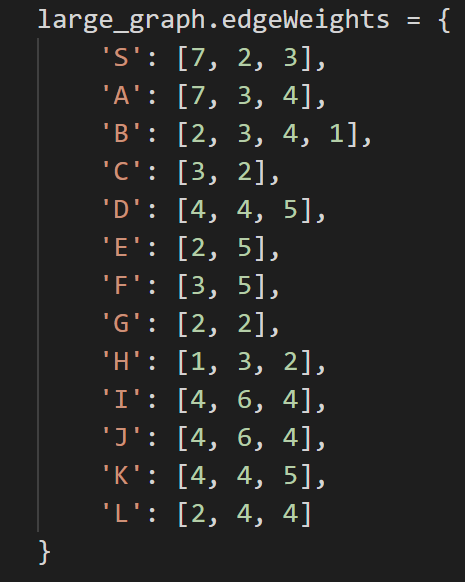
\includegraphics[width=0.8\textwidth]{large_graph_UCS_visual.png} %0.5指图片宽度
		
	\end{minipage}%
	\caption{large graph}
\end{figure}

\begin{figure}[h]
	\centering
	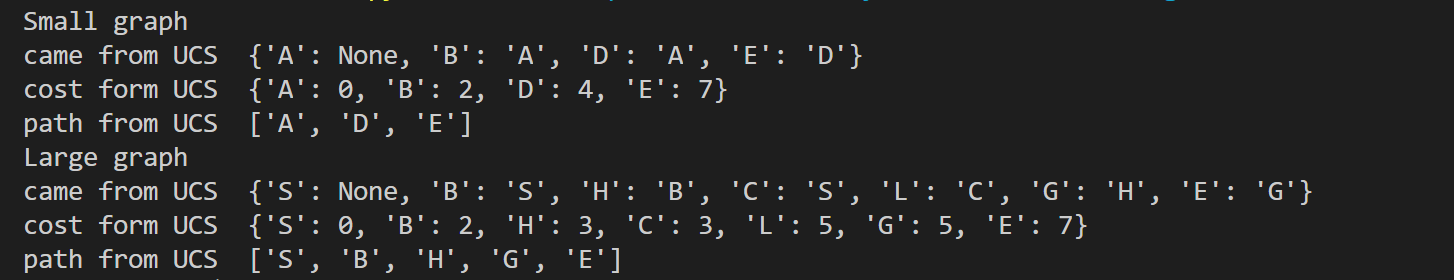
\includegraphics[width=1\textwidth]{UCS_result.png}
	\caption{result for UCS}
	\label{fig:label}
\end{figure}



\subsection{\emph{AStarSearch.py}}

The graphs are same as the previous graphs.
\begin{figure}[h]
	\centering
	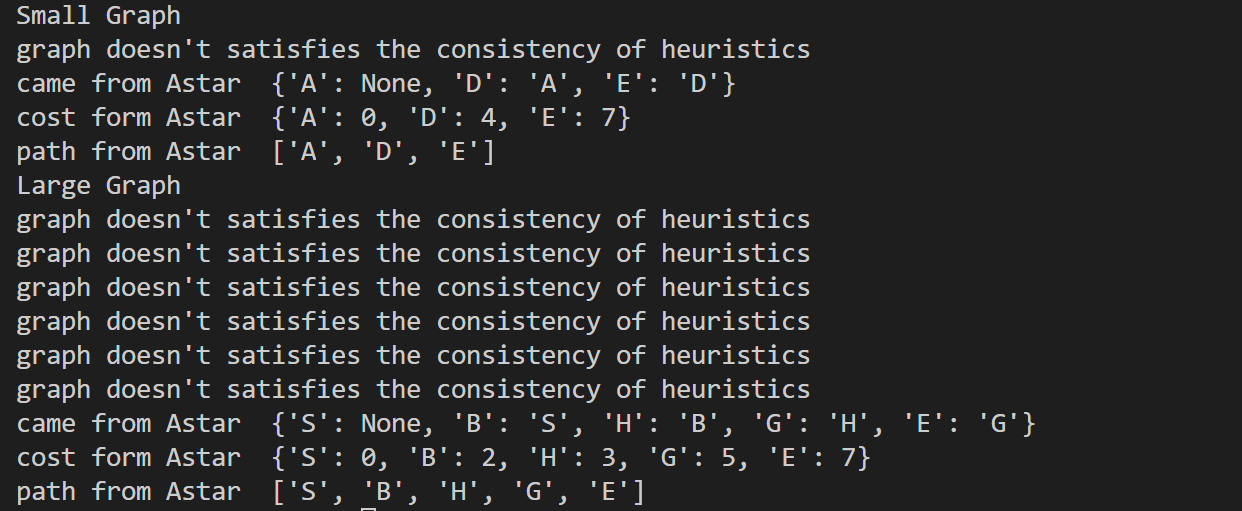
\includegraphics[width=1\textwidth]{AstarResult.png}
	\caption{result for A*}
	\label{fig:label}
\end{figure}

	% You can refer to this set of images by using \ref{fig:oscil}.  ie "please refer to Figure \ref{fig:oscil}."
	% You can refer to a specific subimage by using \ref{fig:Per6A}. ie "please refer to Figure \ref{fig:Per6A}."
   % I prefer the quality of a .png image, but you may use other extensions such as .jpg.


%%%%%%%%%%%%%%%%%%%%%%%%%%%%%%
%%%%%%%%%%%%%%%%%%%%%%%%%%%%%%
\newpage







\section{Discussion \& Conclusion}

Homework1 is more difficult than HW0. I really spent lots of time on the homework. During the process of learning, I 
made many mistakes, which help me further understand the algorithms involved. The most inspiring thing is that I successfully 
solve the A* Search problem in Q3 by writing code. The process is pretty hard but I enjoyed it.
\section{Appendix}

\subsection{code of \emph{Q3.py}}
\begin{lstlisting}
	from queue import PriorityQueue
	import math

	class Graph:
		"""
		Defines a graph with edges, each edge is treated as dictionary
		look up. function neighbors pass in an id and returns a list of 
		neighboring node
		
		"""
		def __init__(self):
			self.locations = {}

	def heuristic(graph, node, target = [5,2]):
		distance = abs(graph.locations['({},{})'.format(node[0],node[1])][0]-target[0]) + abs(graph.locations['({},{})'.format(node[0],node[1])][1]-target[1])
		return distance

	def reconstruct_path(came_from, start, goal):

		path = []
		current_node = goal
		while(came_from[current_node] is not None):
			path.append(current_node)
			# print(current_node)
			if came_from[current_node] is  None :
				break
			current_node = '({},{})'.format( came_from[current_node][0],came_from[current_node][1])
		path.append(current_node)
		path.reverse()
		return path

	def AstarSearch(graph, start = [1,2], target = [5,2]):
		came_from = {} # key is child and value is father
		cost_so_far = {}
		
		came_from['({},{})'.format(start[0],start[1])] = None
		cost_so_far['({},{})'.format(start[0],start[1])] = 0

		closed_set = [start]
		Astar_queue = PriorityQueue(maxsize=0)
		Astar_queue.put((0 + heuristic(graph,start), [None, start, 0]))

		step = 0

		while not Astar_queue.empty():
			Expand = Astar_queue.get()
			if Expand[1][1] in closed_set and step is not 0:  
				continue

			step+=1
			print('\item '+"step "+ str(step))
			print(Expand[1][1])
			print('\n')

			closed_set.append(Expand[1][1])
			came_from['({},{})'.format(Expand[1][1][0],Expand[1][1][1])] = Expand[1][0]
			cost_so_far['({},{})'.format(Expand[1][1][0],Expand[1][1][1])] = Expand[1][2]

			if (Expand[1][1][0] is target[0])  and (Expand[1][1][1] is target[1]) :
				return came_from,cost_so_far
			
			for i in [-1,0,1]:
				for j in [-1,0,1]:
					if abs(i+j) is not 1 :
						continue
					next_node = [Expand[1][1][0]+i, Expand[1][1][1]+j]
					if (next_node not in closed_set) and ( '({},{})'.format(next_node[0],next_node[1]) in graph.locations):
						Astar_queue.put((1+Expand[1][2]+heuristic(graph,next_node), [Expand[1][1], next_node, 1+Expand[1][2]]))
						
			print('fringe list')
			print(Astar_queue.queue)
			print('\n')
			print('closed set')
			print(closed_set)
			print('\n')

		return came_from,cost_so_far
		

	if __name__=="__main__":
		graph = Graph()
		for i in range (0,7):
			for j in range (0,5):
				graph.locations['({},{})'.format(i,j)] = [i, j]
		
		del graph.locations['(3,1)']
		del graph.locations['(3,2)']
		del graph.locations['(3,3)']

		came_from, cost_so_far =  AstarSearch(graph)

		path = reconstruct_path(came_from,"(1,2)","(5,2)")

		print('final path ')
		print(path)


\end{lstlisting}


\end{document} % DONE WITH DOCUMENT!


%%%%%%%%%%
PERSONAL FAVORITE LAB WRITE-UP STRUCTURE
%%%%%%%%%%
\section{Introduction}
	% No Text Here
	\subsection{Purpose}
		% Lab objective
	\subsection{Equipment}
		% Any and all equipment used (specific!)
	\subsection{Procedure}
		% Overview of the procedure taken (not-so-specific!)
\newpage
\section{Schematic Diagrams}
	% Any schematics, screenshots, block
   % diagrams used.  Possibly photos or
	% images could go here as well.
\newpage
\section{Experiment Data}
	% Depending on lab, program code would be
	% included here without the Estimated and
	% Actual Results.
	\subsection{Estimated Results}
		% Calculated. What it should be.
	\subsection{Actual Results}
		% Measured.  What it actually was.
\newpage
\section{Discussion \& Conclusion}
	% 3 Paragraphs:
		% Restate the objective of the lab
		% Discuss personal trials, errors, and difficulties
		% Conclude the lab


%%%%%%%%%%%%%%%%
COMMON COMMANDS:
%%%%%%%%%%%%%%%%
% IMAGES
begin{figure}[H]
   \begin{center}
      \includegraphics[width=0.6\textwidth]{RTL_SCHEM.png}
   \end{center}
\caption{A screenshot of the RTL Schematics produced from the Verilog code.}
\label{RTL}
\end{figure}

% SUBFIGURES IMAGES
\begin{figure}[H]
  \centering
  \subfloat[LED4 Period]{\label{fig:Per4}\includegraphics[width=0.4\textwidth]{period_led4.png}} \\
  \subfloat[LED5 Period]{\label{fig:Per5}\includegraphics[width=0.4\textwidth]{period_led5.png}}
  \subfloat[LED6 Period]{\label{fig:Per6}\includegraphics[width=0.4\textwidth]{period_led6.png}}
  \caption{Period of LED blink rate captured by osciliscope.}
  \label{fig:oscil}
\end{figure}

% INSERT SOURCE CODE
\lstset{language=Verilog, tabsize=3, backgroundcolor=\color{mygrey}, basicstyle=\small, commentstyle=\color{BrickRed}}
\lstinputlisting{MODULE.v}

% TEXT TABLE
\begin{table}
\begin{center}
\begin{tabular}{|l|c|c|l|}
	x & x & x & x \\ \hline
	x & x & x & x \\
	x & x & x & x \\ \hline
\end{tabular}
\caption{Caption}
\label{label}
\end{center}
\end{table}

% MATHMATICAL ENVIRONMENT
$ 8 = 2 \times 4 $

% CENTERED FORMULA
\[  \]

% NUMBERED EQUATION
\begin{equation}
	
\end{equation}

% ARRAY OF EQUATIONS (The splat supresses the numbering)
\begin{align*}
	
\end{align*}

% NUMBERED ARRAY OF EQUATIONS
\begin{align}
	
\end{align}

% ACCENTS
\dot{x} % dot
\ddot{x} % double dot
\bar{x} % bar
\tilde{x} % tilde
\vec{x} % vector
\hat{x} % hat
\acute{x} % acute
\grave{x} % grave
\breve{x} % breve
\check{x} % dot (cowboy hat)

% FONTS
\mathrm{text} % roman
\mathsf{text} % sans serif
\mathtt{text} % Typewriter
\mathbb{text} % Blackboard bold
\mathcal{text} % Caligraphy
\mathfrak{text} % Fraktur

\textbf{text} % bold
\textit{text} % italic
\textsl{text} % slanted
\textsc{text} % small caps
\texttt{text} % typewriter
\underline{text} % underline
\emph{text} % emphasized

\begin{tiny}text\end{tiny} % Tiny
\begin{scriptsize}text\end{scriptsize} % Script Size
\begin{footnotesize}text\end{footnotesize} % Footnote Size
\begin{small}text\end{small} % Small
\begin{normalsize}text\end{normalsize} % Normal Size
\begin{large}text\end{large} % Large
\begin{Large}text\end{Large} % Larger
\begin{LARGE}text\end{LARGE} % Very Large
\begin{huge}text\end{huge}   % Huge
\begin{Huge}text\end{Huge}   % Very Huge


% GENERATE TABLE OF CONTENTS AND/OR TABLE OF FIGURES
% These seem to have some issues with the "revtex4" document class.  To use, change
% the very first line of this document to "article" like this:
% \documentclass[aps,letterpaper,10pt]{article}
\tableofcontents
\listoffigures
\listoftables

% INCLUDE A HYPERLINK OR URL
\url{http://www.derekhildreth.com}
\href{http://www.derekhildreth.com}{Derek Hildreth's Website}

% FOR MORE, REFER TO THE "LINUX CHEAT SHEET.PDF" FILE INCLUDED!
